\section{Experiments}
\label{sec:exp}



\begin{figure}
{\footnotesize
\begin{tabular*}{3.5in}{l|ccc}
Cluster & Sapling & Viz & Keeneland \\
\midrule
Nodes   &   4     &  10 &  32 (120) \\
CPUs/Node & 2x Xeon 5680 & 2x Xeon 5680 & 2x Xeon 5660 \\
HyperThreading & on & off & off \\
GPUs/Node & 2x Tesla C2070 & 5x Quadro Q5000 & 3x Tesla M2090 \\
DRAM/Node & 48 GB & 24 GB & 24 GB \\
Infiniband & 2x QDR & QDR & 2x QDR \\
\end{tabular*}
}
\vspace{-2mm}
\caption{System configurations used for the experiments. \label{fig:systems}}
\vspace{-6mm}
\end{figure}

% FIXME
% This is a nice paragraph, but it doesn't belong here; perhaps in the mapping section
% if we have space.
%
%Nodes with multiple instances of different resources are challenging
%for existing programming models with flat system views (e.g., MPI).
%They must either lump resources together and ignore internal irregularities (e.g. NUMA
%in multi-socket x86 systems), or divide a single physical node into
%multiple smaller nodes, ignoring the better affinity between sockets/GPUs/etc.
%on the same node. In contrast, the machine model used by Legion is based on an
%affinity graph of CPUs and GPUs and accurately captures complex
%machine hierarchies.
%
% FIXME
%   I cut this from the above, commented-out paragraph because it was a digression. 
%  
% and either wasting or over-subscribing some resources when
%the quantities of different resources don't share a common divisor.


We evaluate the efficiency and scalability of Legion using
three applications on three clusters (see Figure~\ref{fig:systems}).  All three
clusters were Linux-based, and the Legion runtime was built using pthreads for
managing CPU threads, CUDA\cite{CUDA} for GPUs, and GASNet\cite{GASNET07} for
inter-node communication.  The RDMA features of GASNet were used to create a 
globally addressable, but relatively slow, {\em GASNet memory} that is accessible
by all nodes.
For each application, multiple problem sizes were used, and each size problem was
run on subsets of each machine ranging from the smallest (a single CPU core or GPU)
to the largest or near-largest (except Keeneland, where we limited
runs to 32 nodes to get sufficient cluster time).
By examining performance of the same size problem over progressively larger
machines, we measure Legion's strong scaling.
By increasing the problem size as well, we also measure weak scaling.

\subsection{Circuit Simulation}
\label{subsec:exp_ckt}

The first experiment we investigate is the distributed circuit simulation described in 
Section~\ref{sec:ex}.  The Legion SOOP runtime handles all of the resource allocation, 
scheduling, and data movement across the cluster of GPUs.  In particular,  
Legion's ability to efficiently move the irregularly partitioned
shared data around the system while keeping the private nodes and wires resident in
each GPU's framebuffer memory is critical to achieving good scalability.

Circuits of two different sizes were simulated.  The first had 480K wires, connecting
120K nodes.  The second is twice as large, with nearly 1M wires connecting 
250K nodes.  In addition to running these tests on varying numbers of
nodes, the number of GPUs used by the runtime was also varied.  In no case did the 
changes to nodes or number of GPUs per node require changes to the application code.

The circuit simulation has a simple application-specific mapper.  At initialization
time, the mapper queries the list of GPUs in the machine and identifies each GPU's
framebuffer memory and {\em zero-copy} memory (pinned memory that both the GPUs and
CPUs on a node can access directly).  Once the circuit is partitioned, the partitions
are assigned a home GPU in round-robin fashion.  Every task related to that partition is
then sent to the home GPU, with no task stealing allowed.  
(In a well-partitioned circuit,
load imbalance is low enough that the cost of moving the private data for a piece from one
GPU to another outweighs any benefits.)

  The regions for the tasks are mapped as 
shown in Figure~\ref{fig:gpumapping}.  Wires and private node data are kept in each GPU's
framebuffer at all times.  An instance of the all-shared-nodes region is placed in
GASNet memory and instances for just the shared and ghost nodes needed by each GPU
are placed into that GPU's zero-copy memory.  This enables the application kernels
to access the data as well as the necessary inter-node exchanges of data via the GASNet
memory.

\begin{figure}
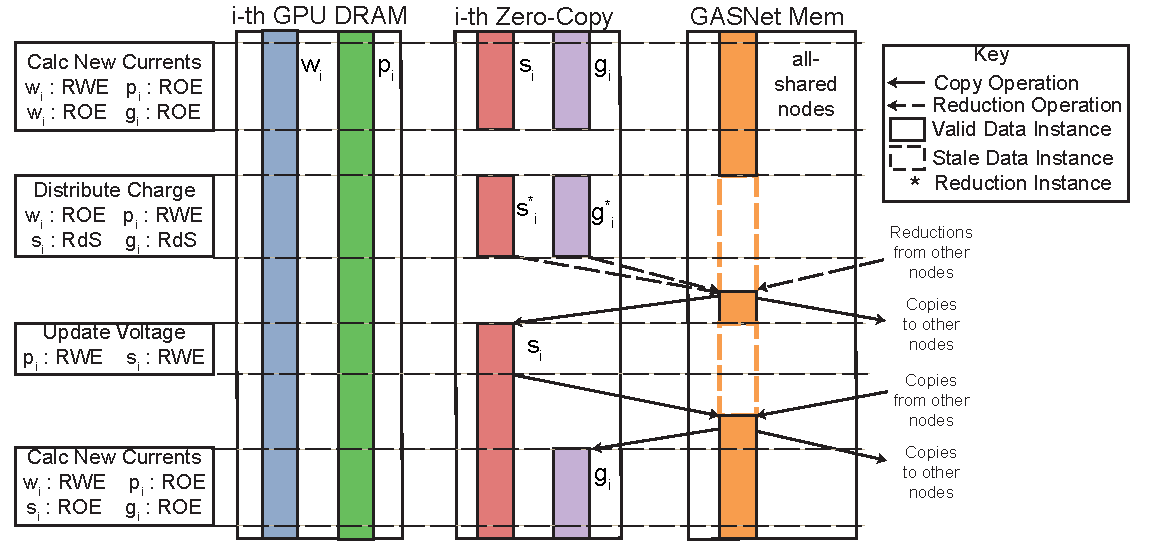
\includegraphics[scale=0.48]{figs/CircuitMem.pdf}
\caption{Tasks and data for the circuit simulation on a cluster of GPUs.}
\label{fig:gpumapping}
\end{figure}

Figure~\ref{fig:ckt_speed} shows the performance of the Legion circuit simulation relative
to a hand-coded single-GPU implementation written in CUDA.  The hand-coded implementation is
able to keep the entire simulation state in fast framebuffer memory.  Each line shows the scaling of
a particular problem size as the number of nodes is varied.  Our results demonstrate
excellent strong scaling, with speedups of 39.0X for the small problem on 48 GPUs and 
62.5X for the larger problem size on 96 GPUs.  The inset in the graph shows the relative
performance for small numbers of GPUs.  On a single GPU, our Legion implementation
is within 5\% of the performance of the hand-coded simulation.

Figure~\ref{fig:ckt_overhead} shows the fraction of the overall simulation time (summed over
all nodes) spent in the application kernels compared to the various pieces of the Legion
SOOP runtime.  As the node count increases, the non-communication overhead stays relatively constant.
As expected the communication overhead grow linearly with number of nodes.

\begin{figure}
\subfigure[Circuit simulation speed relative to single-GPU implementation.]
{
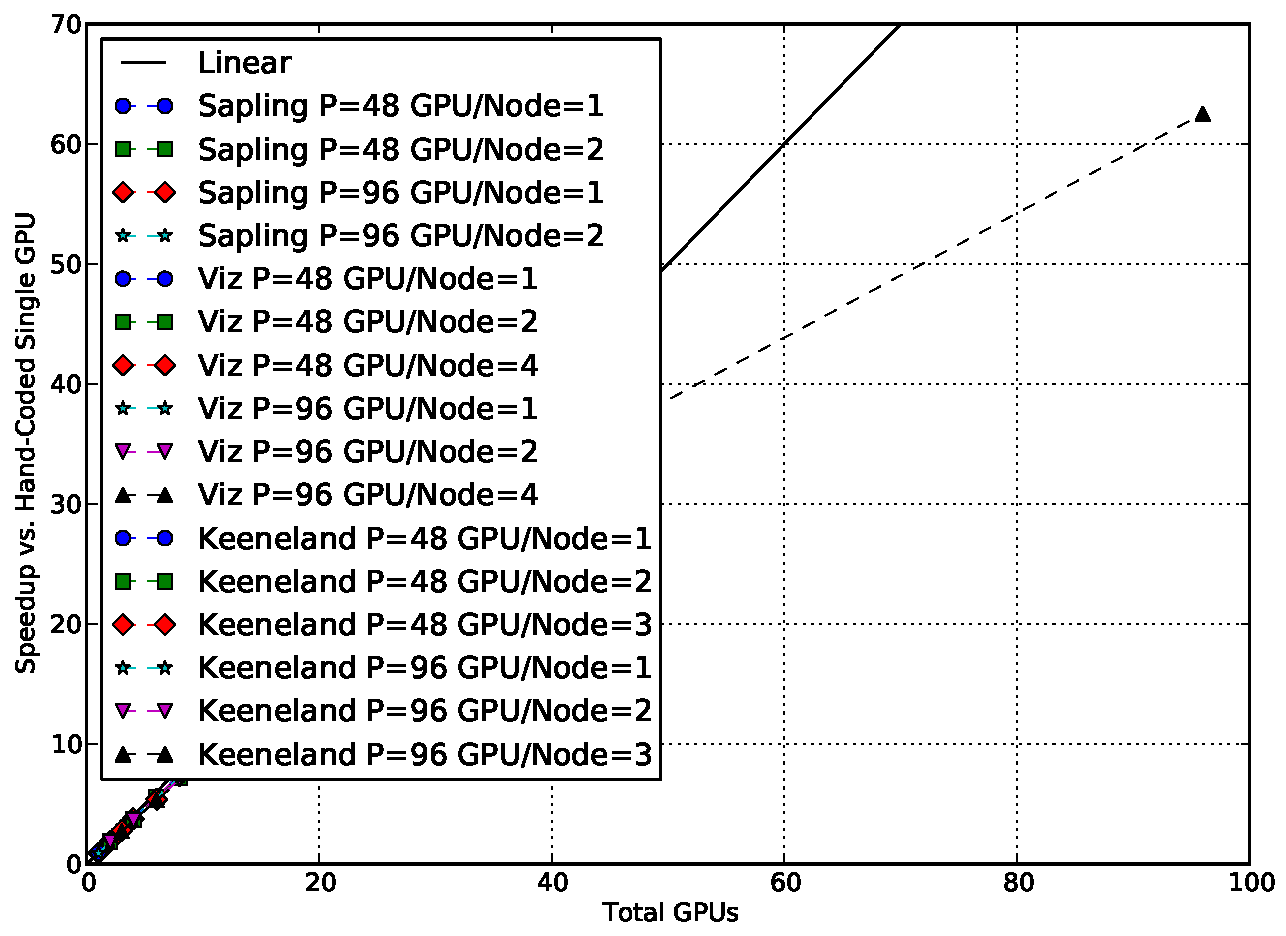
\includegraphics[scale=0.4]{figs/circuit_speedups.pdf}
\makebox[0pt][r]{
\raisebox{0.25 in}{
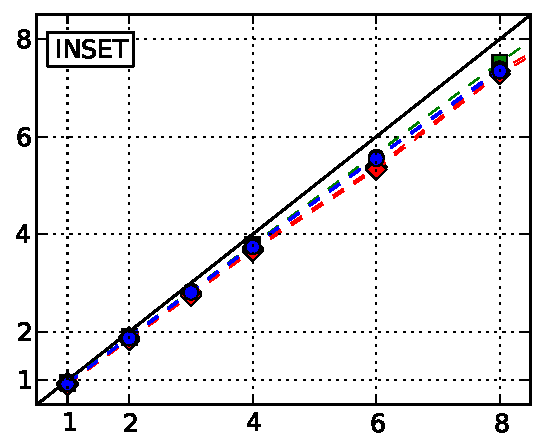
\includegraphics[scale=0.4]{figs/circuit_speedups_zoom.pdf}
}
}
\label{fig:ckt_speed}
}

\subfigure[Overhead of circuit simulation on Keeneland with 3 GPUs/node.]
{
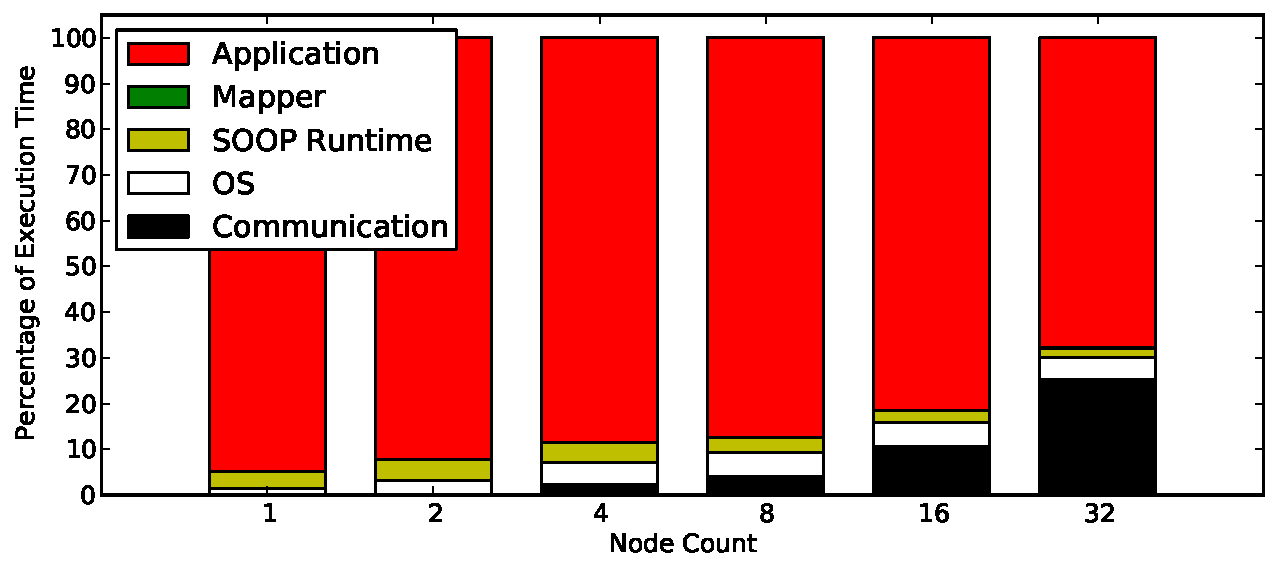
\includegraphics[scale=0.4]{figs/circuit_overhead.pdf}
\label{fig:ckt_overhead}
}
\vspace{-2mm}
\caption{Circuit simulation results.}
\vspace{-6mm}
\end{figure}

\subsection{Particle Simulation}
\label{subsec:exp_fluid}

Our second experiment is a port of the \emph{fluidanimate} benchmark
from the PARSEC benchmark suite\cite{bienia11benchmarking}, which does a
particle-based simulation of an incompressible fluid.  Each particle
interacts only with nearby particles. The benchmark divides the
space in which the fluid can move into a three-dimensional array of
cells such that the range of interaction is limited to just the cells
adjacent (including diagonals) to the one a particle resides in.  The
application divides the array into {\em grids} and assigns each grid to
a thread.  Per-particle locking safely accesses particles in
cells that lie on the edge of a grid.  This fine-grained locking
scheme along with the assumption of a shared address space gives
good scaling in a multicore processor, but prohibits running
beyond a single node.

To extend the scaling further, our port uses region partitioning to
divide the array into grids in a similar way, but avoids relying
on shared memory to handle interactions between grids.
Instead, the Legion version creates
explicit ghost copies of cells on grid boundaries and uses
those ghost cells to exchange information between the grids.

The particle simulation's mapper is very simple: it maps one grid's
tasks onto each processor and maps all that grid's regions (both
internal and ghost regions) into that processor's system memory.  The
exchange of ghost cell data between processors is handled by the
Legion runtime as a ghost cell region is alternately mapped to two
different memories.

Figure~\ref{fig:fluid_single} compares the performance of the Legion
implementation against the PARSEC version, using a relatively small
problem (300K particles on a 15x21x15 array of cells).  Speedups for
both the Legion and threaded PARSEC implementations are measured 
relative to PARSEC's serial version, which eliminates all locking
operations.  Between 1 and
4 threads, the PARSEC and Legion results are nearly indistinguishable,
indicating neither the Legion runtime nor the restructuring of the
implementation to allow multi-node scaling impose any significant
overhead.
%It's possible that the use of explicit ghost cells rather than fine-grained sharing of cache lines might be a net win.  
At 8 threads and above, performance begins to vary.  Both the Legion
and PARSEC versions on Viz flatten out as they over-subscribe the 12
physical cores.  On Sapling, which has HyperThreading enabled,
deviations from linear begin sooner as the operating system's
thread placement choices begin to matter.

To measure scaling beyond a single node, three different problem sizes
were run for each of the three systems (Figure~\ref{fig:fluid_multi}).
For the smallest problem (300K particles), we observe a 20\% speedup
from 1 to 2 nodes (16 threads total), but slow
down beyond that due to communication overhead---at 4 nodes there are
twice as many ghost cells as interior grid cells.  The larger problem
sizes (2.4M and 19M particles) do much better, with scaling of up to
5.4x when going from 1 node up to 16 because of a lower
communication-to-computation ratio.

%Although the particle simulation being performed is on a regular array of cells, it turns out that the
%distribution of particles amongst the cells is very irregular.  The simulation models gravity, which points in
%the -Y direction, so the particles are clustered mostly in the lower half of the cell array.  The PARSEC
%implementation works around this imbalance by only slicing the cell array through the X and Z axes, yielding
%grids that are uniformly populated, even if the number of boundary cells (for which locks must be used) is
%increased above the minimum. MORE TEXT NEEDED HERE

\begin{figure}
\subfigure[Single-node particle simulation speed.]
{
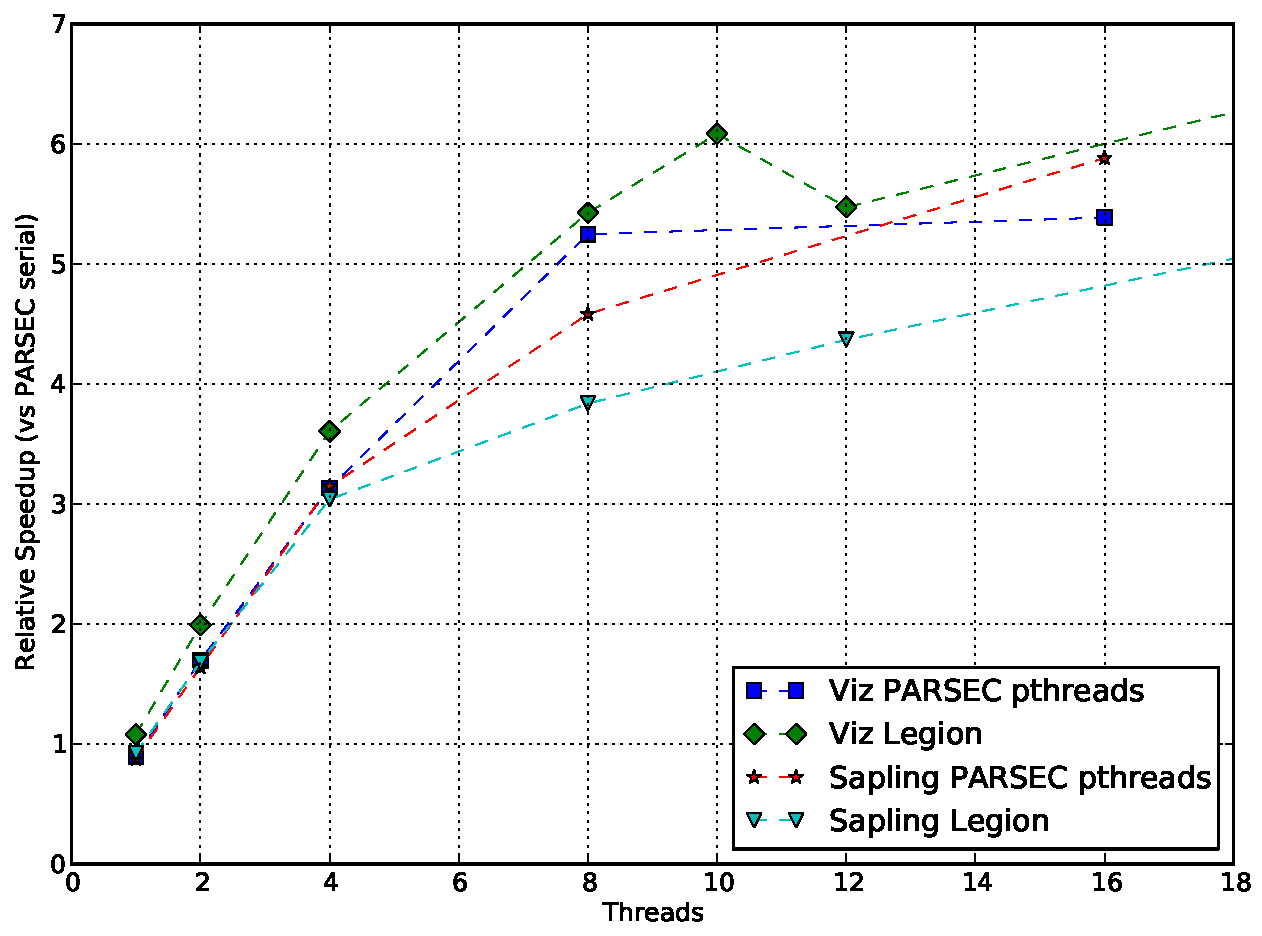
\includegraphics[scale=0.4]{figs/fluid_singlenode.pdf}
\label{fig:fluid_single}
}

\subfigure[Multi-node scaling.]
{
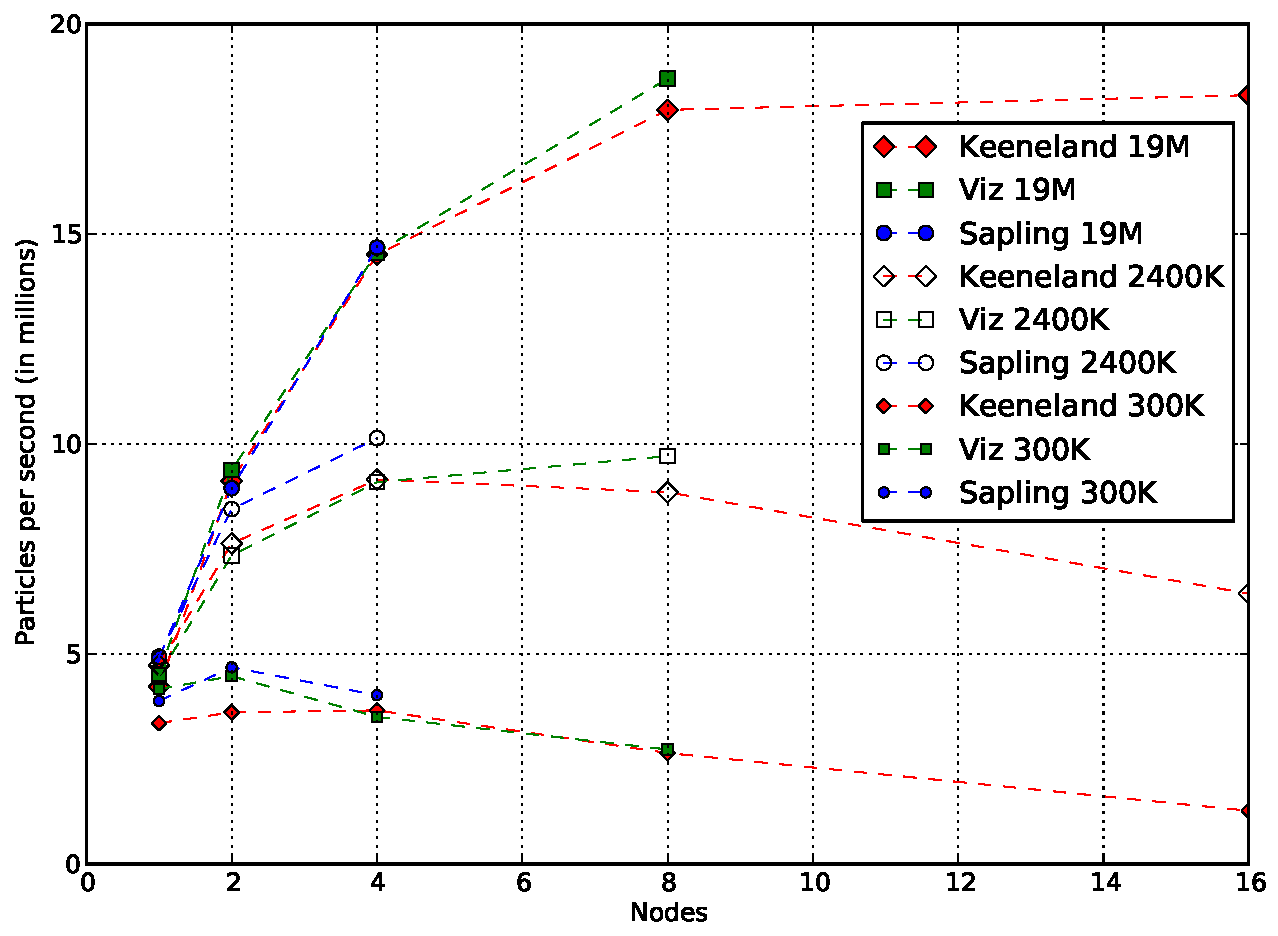
\includegraphics[scale=0.4]{figs/fluid_multinode.pdf}
\label{fig:fluid_multi}
}

%\subfigure[Effect of load-balanced partitioning.]
%{
%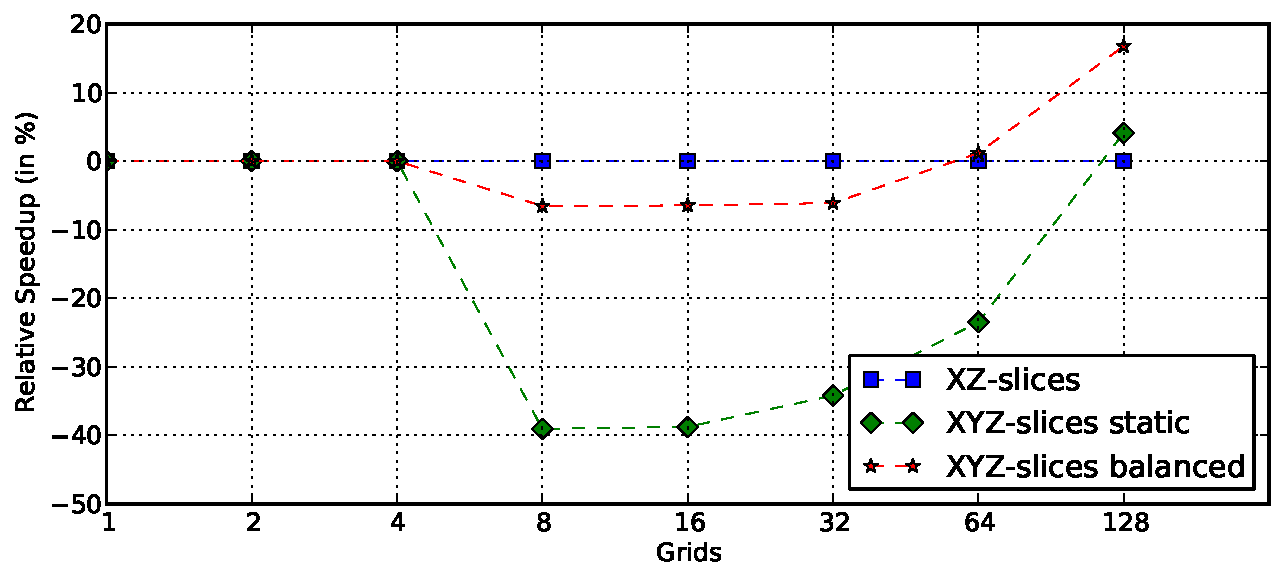
\includegraphics[scale=0.4]{figs/fluid_balance.pdf}
%\label{fig:fluid_balance}
%}
\vspace{-2mm}
\caption{Fluid simulation results.}
\vspace{-6mm}
\end{figure}

\subsection{Adaptive Mesh Refinement}
\label{subsec:exp_amr}
Our final application is based on the third heat equation example from
the Berkeley Labs BoxLib project \cite{BoxLib}.  This application is a
three-level adaptive-mesh-refinement (AMR) code that computes a first
order stencil on a 2D mesh of cells.  
%The simulation iterates for many time steps.  
Updating the simulation for one time step consists of
three phases.  In the first phase, the boundary cells around a box at
a refined level linearly interpolate their values from the nearby
cells at the next coarser level.  The second phase performs the
stencil computation on each cell in every level.  In the third phase,
cells at a coarser level that have been refined are restricted to the
average of the cells that they physically contain at the next finest
level of refinement.

Achieving high-performance on this application is particularly
challenging for several reasons.  First, the application has a very
high communication-to-computation ratio which, for a fixed problem
size, begins as being memory bound and with increasing node count
becomes network bound as the perimeter-to-area ratio of cell grids
increases.  Second, when choosing how to partition cells into grids,
the programmer must consider the locality between cells within a
level as well as across levels.  For
cross-level cell dependences, optimal mapping decisions can only be made at
runtime as the location of refinements are dynamically determined.
Finally, this application has parallelism both
between tasks running at the same level and tasks running across
levels, leading to complicated input-dependent data dependences.

BoxLib's implementation partitions cells within a level 
into a number of grids based on the number of nodes in the
machine and distributes one grid from each level to each node.  This
optimizes for memory bandwidth and load balance, but does not 
exploit cross-level locality between grids from
different levels of refinement.  Furthermore, BoxLib does not block
grids into sub-grids to take advantage of intra-grid locality.

Our Legion implementation performs two optimizations that allow us to
outperform BoxLib.  First, for each level of
refinement we recursively partition the logical region of cells based
on the number of nodes in the machine and the sizes of the L2 and L3 caches.
%Legion allows us to describe locality for many levels of
%the memory hierarchy instead of just at the node-level.
Our second optimization takes advantage of the cross-level locality.
We wrote an application-specific mapper that dynamically discovers
relationships between grids at different levels of refinement.  The
mapper dynamically performs intersection tests between logical regions
containing grids of different refinement levels.  If the mapper
discovers overlaps between grids from different levels, the mapper
places them on the same node in the machine.  The
mapper memoizes the intersection tests to amortize their cost.  The
mapper also dynamically load balances by distributing unconstrained
grids from the coarsest level onto under-loaded nodes.

We compared our Legion implementation against BoxLib on three
different problem sizes with a fixed number of cells per level of
refinement, but with randomly chosen refinement locations.  BoxLib
also supports OpenMP and we took their best performance from using 1,
2, 4, or 8 threads per node.  Our Legion implementation always uses
one thread per node to illustrate that in this application locality is
significantly more important than fine-grained data-parallelism.  

Figure~\ref{fig:amr_total} gives the results.
On just one node, blocking for caches using Legion achieves up to 2.6X
speedup over BoxLib.  As node count increases, the mapper's
ability to exploit cross-level locality further increases
the performance advantage to 5.4X by reducing the total
communication costs.

As the node count increases the AMR code becomes highly dependent on
interconnect performance.  BoxLib performs much better on Keeneland
than on Viz due to the better interconnect.  
At higher node counts BoxLib
begins to catch up (see Figure~\ref{fig:amr_keeneland})
because our application's intra-level ghost-cell exchange algorithm
uses GASNet memory to communicate ghost cells, requiring a
linear increase in network traffic with the number of nodes.  BoxLib
uses direct node-to-node exchanges of ghost cells, similar to
our fluid application.  A future implementation of our AMR code will
employ a similar ghost cell exchange algorithm to improve scalability.

\begin{figure}
\subfigure[Sapling results.]
{
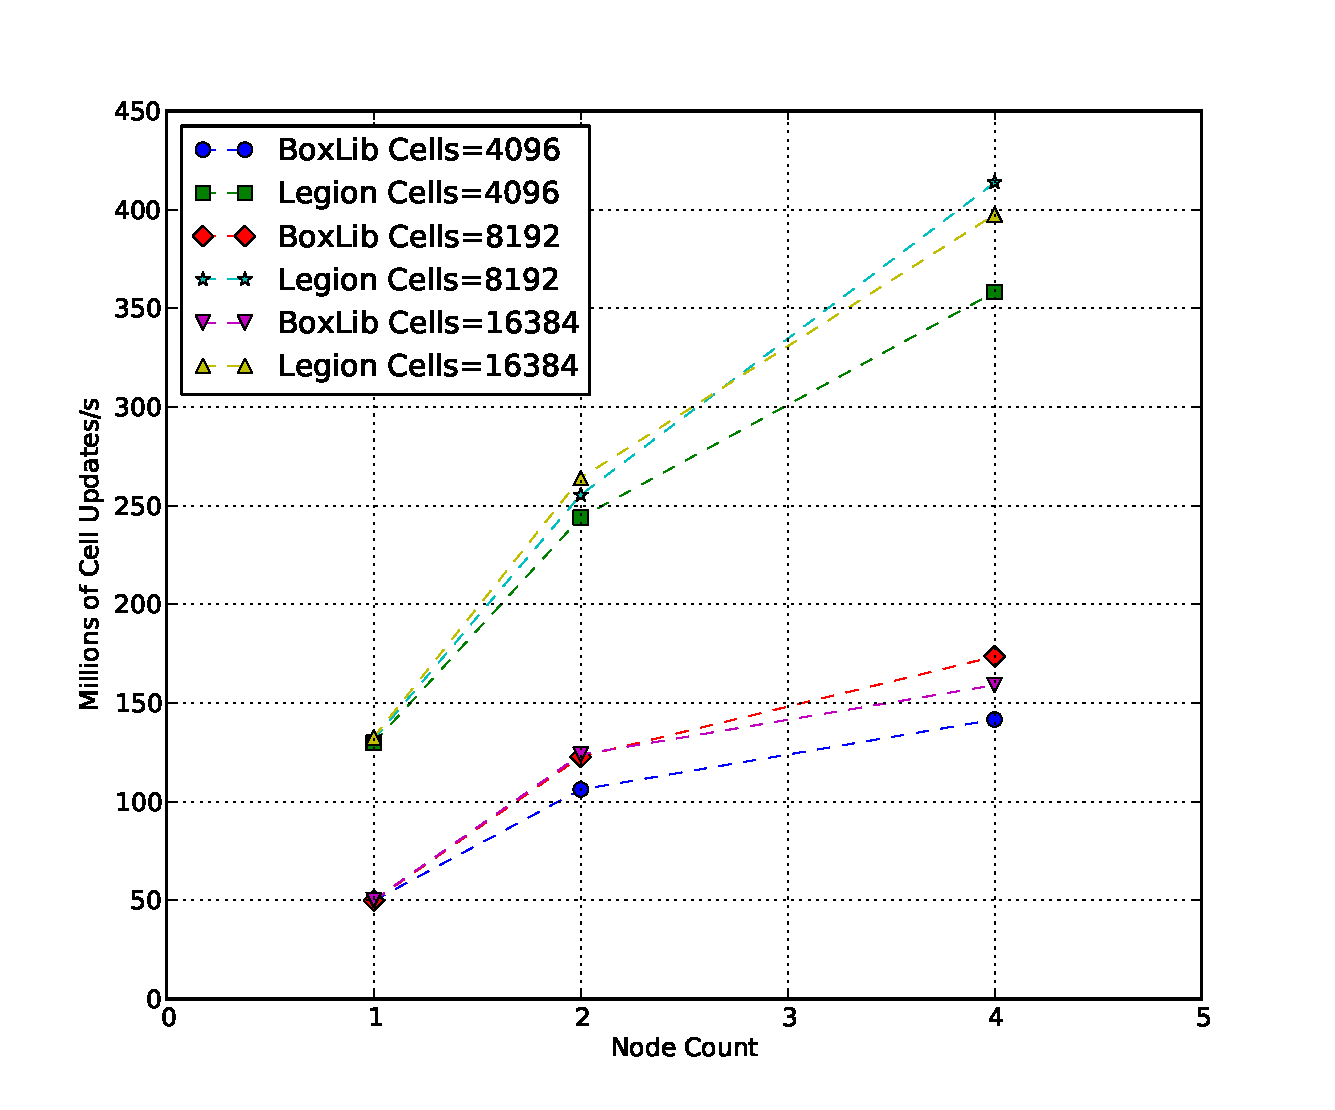
\includegraphics[scale=0.4]{figs/Sapling_amr.pdf}
\label{fig:amr_sapling}
}

\subfigure[Viz results.]
{
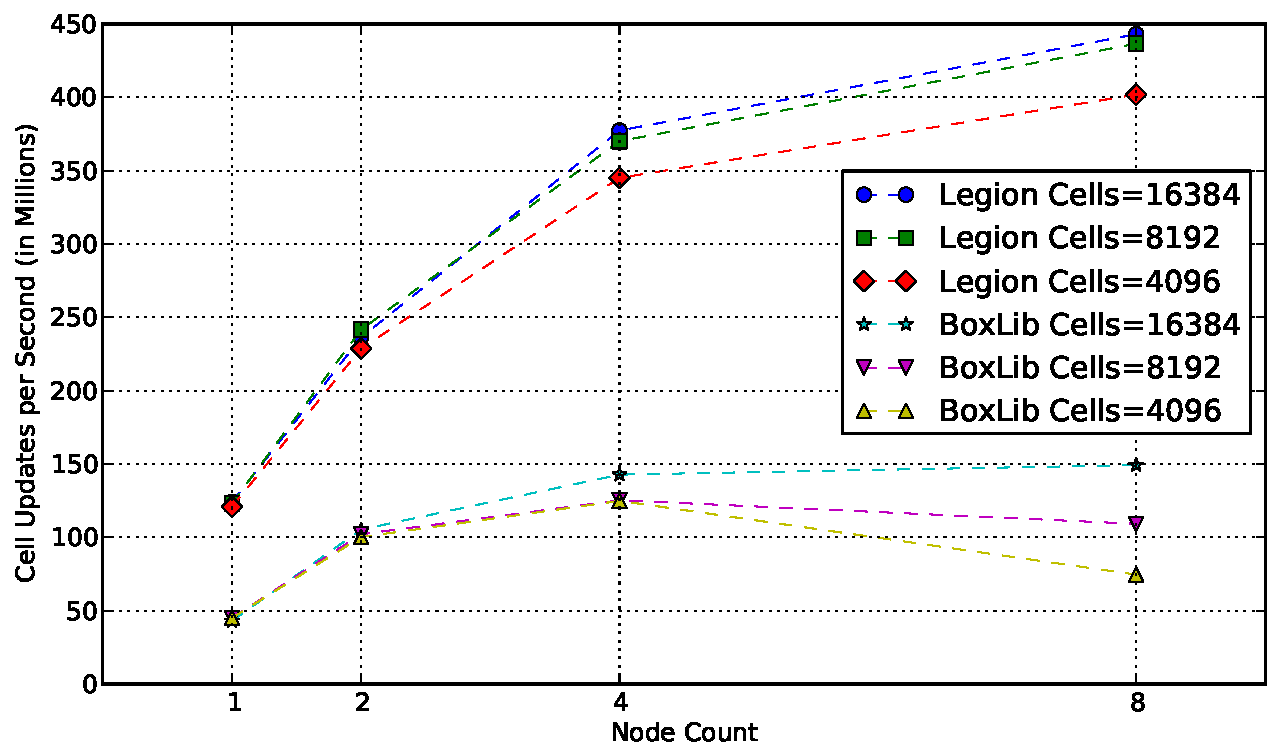
\includegraphics[scale=0.4]{figs/Viz_amr.pdf}
\label{fig:amr_viz}
}

\subfigure[Keeneland results.]
{
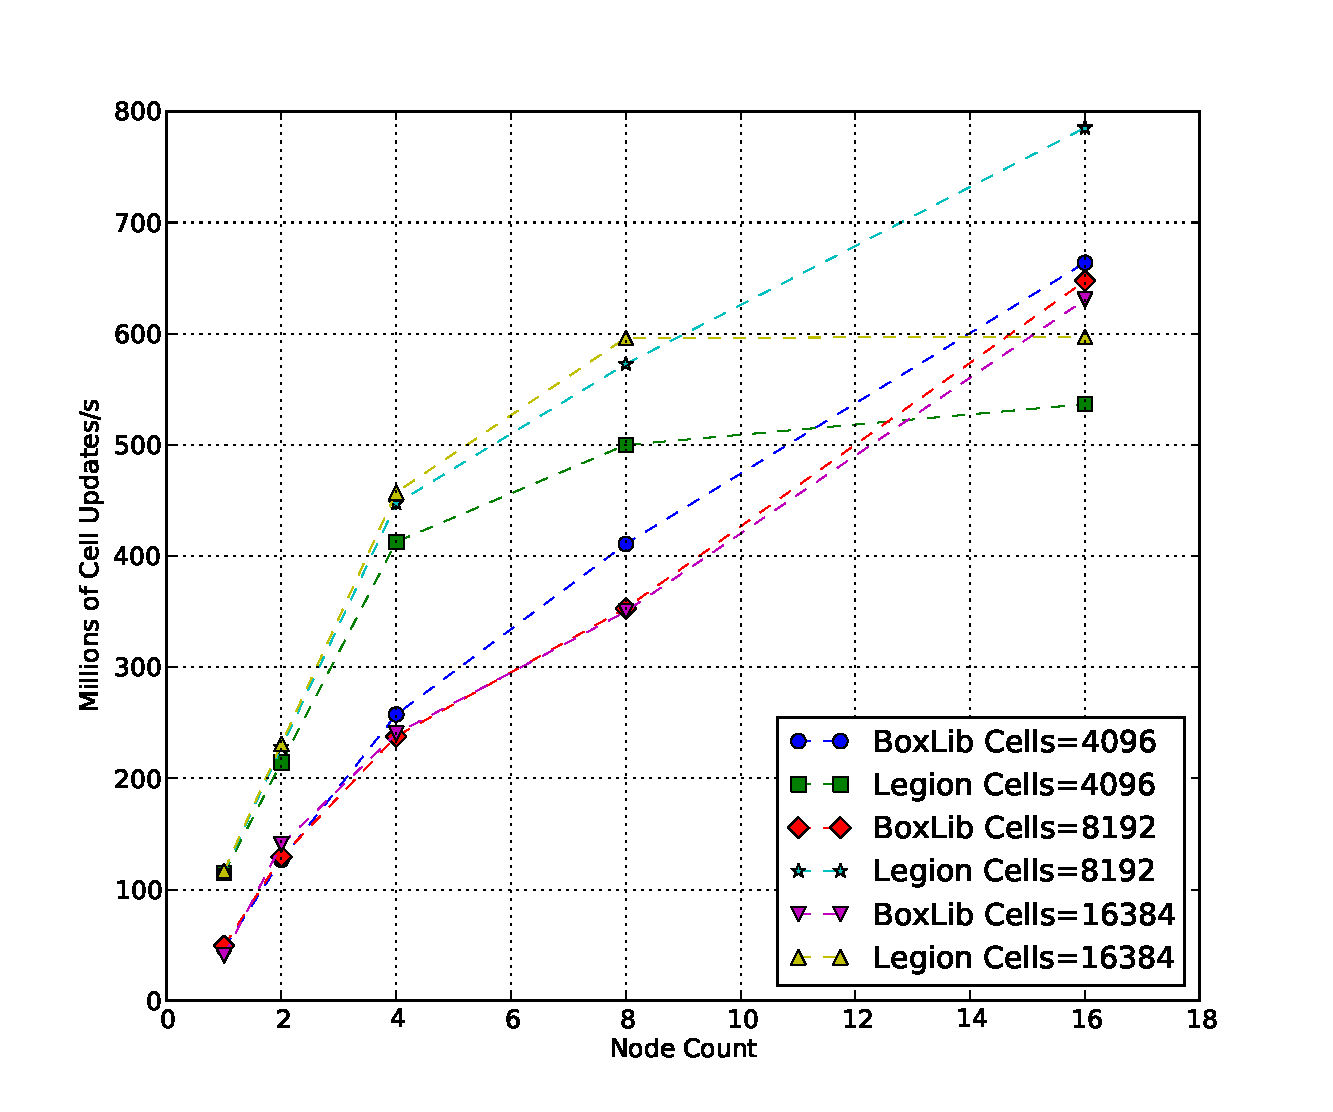
\includegraphics[scale=0.4]{figs/Keeneland_amr.pdf}
\label{fig:amr_keeneland}
}
\vspace{-2mm}
\caption{Throughput of adaptive mesh refinement code. \label{fig:amr_total}}
\vspace{-6mm}
\end{figure}
